\documentclass[12pt, titlepage]{article}

\usepackage{booktabs}
\usepackage{tabularx}
\usepackage{hyperref}
\hypersetup{
    colorlinks,
    citecolor=black,
    filecolor=black,
    linkcolor=red,
    urlcolor=blue
}
\usepackage[round]{natbib}
\usepackage{tikz}
\usepackage{graphicx}
\usepackage{float}

\input{../Comments}
\input{../Common}

\begin{document}

\title{Verification and Validation Report: \progname}
\author{\authname}
\date{\today}
\maketitle

\pagenumbering{roman}

\section{Revision History}

\begin{tabularx}{\textwidth}{p{3cm}p{2cm}X}
\toprule {\bf Date} & {\bf Version} & {\bf Notes}\\
\midrule
April 16, 2025 & 1.0 & Initial document\\
\bottomrule
\end{tabularx}

~\newpage

\section{Symbols, Abbreviations and Acronyms}

\renewcommand{\arraystretch}{1.2}
\begin{tabular}{l l}
  \toprule
  \textbf{symbol} & \textbf{description}\\
  \midrule
  T & Test\\
  \bottomrule
\end{tabular}\\

\wss{symbols, abbreviations or acronyms -- you can reference the SRS tables if needed}

\newpage

\tableofcontents

\listoftables %if appropriate

\listoffigures %if appropriate

\newpage

\pagenumbering{arabic}

\section{Functional Requirements Evaluation}
Each functional requirement was evaluated based on the reflection of
implementation presentation and tool's test
results.

The demonstration provided a valuable opportunity to observe how others
interpreted the output of the reconstruction pipeline, leading to adjustments in
the GUI for better visual clarity and confirmation of expected behavior. The
core functionality, Radon transform, filtering, and back-projection, was
tested via unit tests. Results show that expected outputs were generated for
provided synthetic inputs.

\section{Nonfunctional Requirements Evaluation}

\subsection{Usability}
The software features a GUI designed using Tkinter with ttkbootstrap for
enhanced usability. Users can upload images or .h5 files, select reconstruction
methods, and visualize results without manual configuration.

\subsection{Performance}
Performance is constrained by the numerical computations in Fourier filtering
and back-projection. Though not heavily optimized, the runtime remains
acceptable for standard image sizes.

\subsection{Portability, Maintainability, and Reusability}
The system supports multiple platforms and is modularized. Each function is
encapsulated in dedicated modules to enhance maintainability. Filter operations
can be reused for different projection types.

\section{Unit Testing}
Unit testing was performed using pytest. A total of 7 test cases were written and executed:
\begin{figure}[H]
  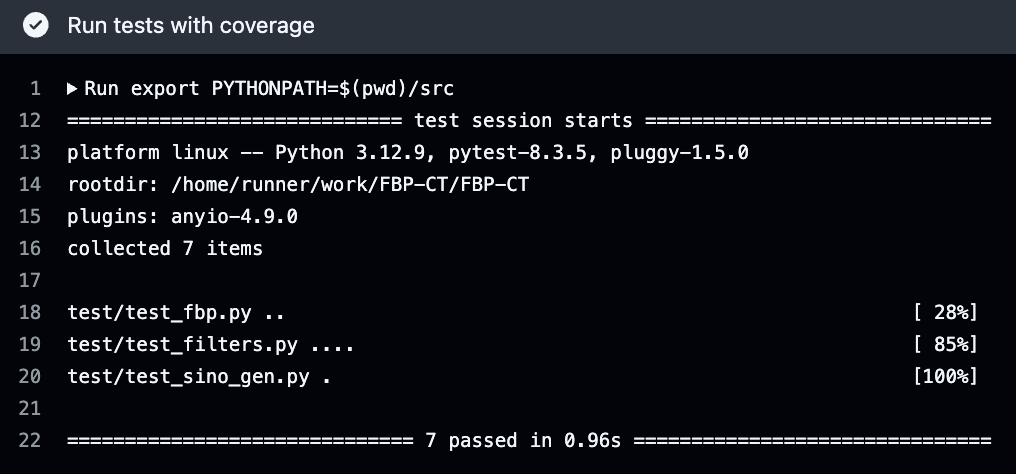
\includegraphics[scale=0.8]{test.png}
\caption{Unit testing results}
\label{test}
\end{figure}

All tests passed successfully, indicating that core functionality such as ramp
filtering and back-projection works correctly for the tested cases.

\section{Changes Due to Testing}
Initial test results highlighted unhandled edge cases and mismatches in data
shape during filtering. Adjustments were made to input validation and
interpolation steps to align inputs and expected outputs. Some utility functions
were also refactored to isolate logic for better testing.

\section{Automated Testing}
Automated testing was conducted using pytest. All test scripts were executed in
Github Actions (as Figure \ref{test}), ensuring continuous integration and
deployment (CI/CD). This setup verifies the system on every commit, reducing the
risk of regression and maintaining code reliability.

\section{Trace to Requirements}
\begin{table}[H]
\centering
\begin{tabular}{|c|c|c|c|}
\hline
  \tikz{\node[below left, inner sep=1pt] (test) {test};%
      \node[above right,inner sep=5pt] (requirement) {requirement};%
      \draw (test.north west|-requirement.north west) -- (test.south east-|requirement.south east);}
   & R1 & R2 & R3  \\
\hline
test\_sino\_gen.py  & X  &    &     \\ \hline
test\_filters.py  &    & X  &     \\ \hline
test\_filters.py  &    &    &  X  \\ \hline
\end{tabular}
\caption{Traceability Matrix Showing the Connections Between Functional Requirements and
  Test Cases}
\label{Table:R_trace}
\end{table}

\section{Trace to Modules}
\begin{table}[H]
\centering
\begin{tabular}{|c|c|c|c|}
\hline
  \tikz{\node[below left, inner sep=1pt] (test) {test};%
      \node[above right,inner sep=5pt] (module) {module};%
      \draw (test.north west|-requirement.north west) -- (test.south east-|requirement.south east);}
   & Simulation & FBP & Filters  \\
\hline
test\_sino\_gen.py  & X  &    &     \\ \hline
test\_filters.py  &    & X  &     \\ \hline
test\_filters.py  &    &    &  X  \\ \hline
\end{tabular}
\caption{Traceability Matrix Showing the Connections Between Behaviour Modules and
  Test Cases}
\label{Table:M_trace}
\end{table}

\newpage
\section{Code Coverage Metrics}
Code coverage was evaluated using the coverage tool.Services and utils modules
is covered when testing the main modules. An HTML report was generated:
\begin{figure}[H]
    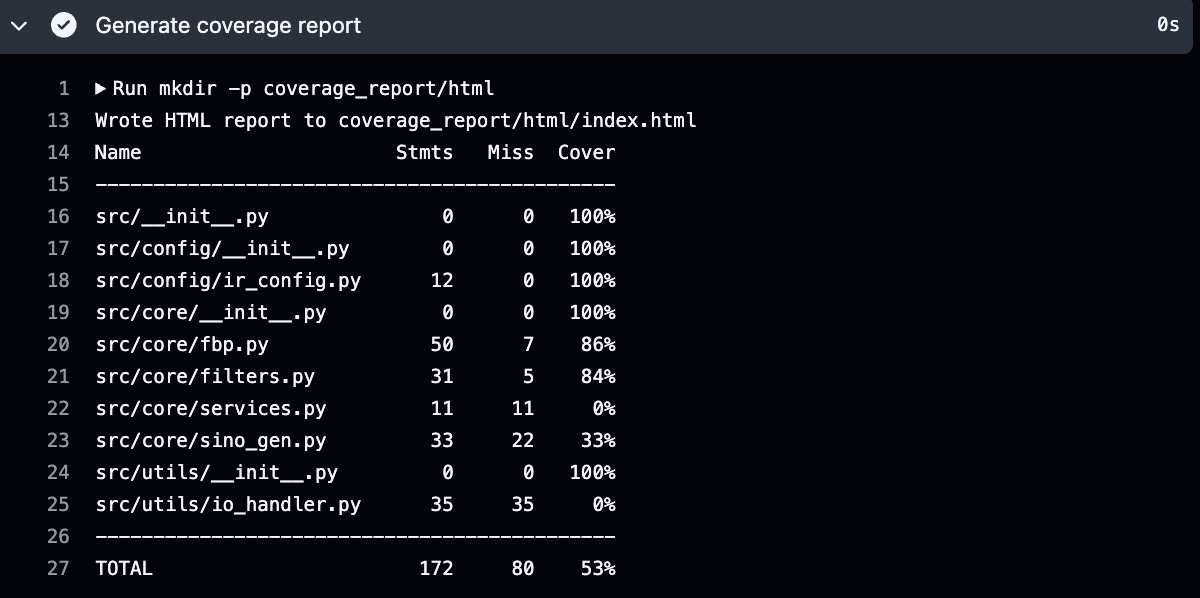
\includegraphics[scale=0.6]{coverage.png}
    \caption{Coverage Report}
    \label{coverage}
\end{figure}

\end{document}
